\chapter{Wstęp}
W archeologii i geologii wiek próbek można określić dzięki wykorzystaniu skaleni. Jest to możliwe dzięki zjawisku stymulowanej luminescencji. Już w latach 60- tych  XX wieku powstał pomysł wykorzystania termoluminescencji, która znalazła wiele zastosowań w archeologii i naukach o Ziemi. Jednym z głównych tematów badań jest datowanie z wykorzystaniem skaleni przy użyciu ich termoluminescencji oraz atermicznym zanikiem luminescencji powodującym zaniżanie daty próbek, który utrudnia datowanie. Atermiczny zanik związany jest z faktem zachodzenia rekombinacji zlokalizowanej, głownie poprzez zachodzące zjawisko tunelowania elektronów z pułapek elektronowych oraz centrów rekombinacyjnych. 

\section{Założenia projektu}
Celem projektu było stworzenie programu symulującego atermiczny zanik sygnału luminescencyjnego w skaleniach. Głównym założeniem było otrzymanie wykresu obrazującego zmianę ilości elektronów znajdujących się w stanie wzbudzonym (znajdujących się w pułapkach) wraz z upływem czasu.

\section{Zjawisko luminescencji w skaleniach}


Jednym ze składników środowiska naturalnego jest promieniowanie jonizujące. Najważniejszym jego źródłem są izotopy promieniotwórcze zawarte w skorupie ziemskiej, atmosferze
i biosferze, emitujące promieniowanie $\alpha$, $\beta$ i $\gamma$. 
W ostatnim okresie, bardzo krótkim w sensie geologicznym oraz historycznym, pojawiły
się nowe jego źródła, związane z działalnością człowieka w zakresie zbrojeń atomowych
i energetyki jądrowej. W dalszym jednak ciągu najważniejszym źródłem promieniowania
jonizującego w środowisku są izotopy promieniotwórcze, które weszły w skład Ziemi w okresie
formowania się układu słonecznego.  Są to przede wszystkim długożyciowe izotopy uranu $U^{238}$, $U^{235}$ i toru $Th^{232}$. Promieniowanie to niesie energię, którą pochłaniają wszystkie substancje występujące
w środowisku - w tym skalenie. Oczywistym jest, że im dłużej substancja  jest poddana promieniowaniu, tym pochłonie jego większą dawkę.

Rzeczywisty kryształ skalenia nie jest idealny. Zawiera on zawsze nieregularności i defekty struktury sieci krystalicznej. Część z nich znajdująca się w paśmie wzbronionym może mieć charakter pułapek, które są zdolne do wychwytywania
elektronów z pasma przewodnictwa i przetrzymywania ich przez długi czas. Stan kryształu, w którym część lub wszystkie pułapki są zapełnione schwytanymi elektronami,
charakteryzuje się nadwyżką energii w porównaniu ze stanem podstawowym.  Nadwyżka ta może zostać wyzwolona i wyemitowana np. w postaci światła. Właśnie to zjawisko wykorzystywane jest jako jedna z metod datowania obiektów archeologicznych
i osadów geologicznych. 
\begin{figure}[h]
\centering
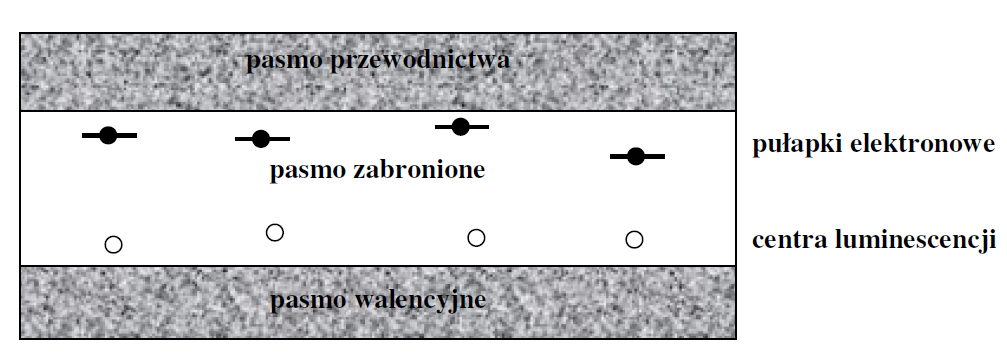
\includegraphics[width=15cm]{strukturapasmowa}
\caption{Struktura pasmowa skalenia. \cite{struktura_pasmowa}}
\label{fig:Struktura pasmowa}
\end{figure}

Zdarza się jednak, że mimo iż uwięziony elektron nie otrzymał dodatkowej energii, będzie w stanie zrekombinować z dziurą. Jest to jest możliwe dzięki  \textbf{zjawisku tunelowania}.

\section{Zjawisko tunelowania}
Tunelowanie, to  proces kwantowo-mechaniczny w którym cząstka ma niezerowe prawdopodobieństwo przejścia przez barierę potencjalną nawet, gdy energia cząstki jest mniejsza od wysokości bariery potencjału.


\begin{figure}[H]
\centering
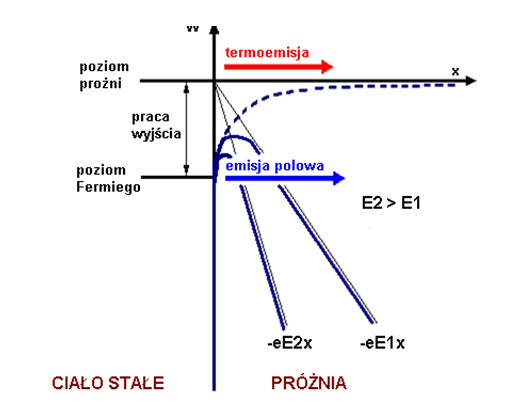
\includegraphics[width=10cm]{tunelowanie}
\caption{Ilustracja mechanizmu emisji polowej. \cite{tunel_pic}}
\label{fig:Tunelowanie}
\end{figure}



W przypadku skaleni prawdopodobieństwo, że elektron nie przetuneluje do centrum rekombinacji wyrażone jest wzorem:
\cite{wzor}
\begin{equation}
\label{eq:1}
P = e^{\frac{-t}{\tau}}
\end{equation}

\begin{equation}
\label{eq:2}
\tau = S^{-1}e^{\alpha r}
\end{equation}


gdzie:
\begin{itemize}
\item t - czas
\item S - stała częstotliwość prób ucieczki
\item $\alpha$ -  stała zależna od różnicy energii pułapki i dziury
\item r - odległość do przetunelowania
\end{itemize}

Wzór \ref{eq:1} wynika z rozwiązania 1D równania Schrödingera z barierą potencjału.





